\documentclass[10pt,a4paper]{article}
\usepackage[T1]{fontenc}
\usepackage[utf8]{inputenc}
\usepackage{lmodern}
\usepackage[margin=18mm,top=18mm,bottom=17mm,headheight=13pt,headsep=6mm,footskip=9mm]{geometry}
\usepackage[table]{xcolor}
\usepackage{microtype}
\usepackage{booktabs,tabularx,array}
\usepackage{enumitem}
\usepackage{titlesec,fancyhdr,lastpage}
\usepackage[skins]{tcolorbox}
\usepackage{tikz}
\usetikzlibrary{arrows.meta,positioning}
\usepackage{hyperref}
\definecolor{navy}{HTML}{17354A}
\definecolor{teal}{HTML}{087E83}
\definecolor{ink}{HTML}{243746}
\definecolor{muted}{HTML}{566873}
\definecolor{pale}{HTML}{EFF5F6}
\definecolor{line}{HTML}{CCDADD}
\definecolor{warm}{HTML}{F5F6F8}
\hypersetup{colorlinks=true,urlcolor=teal,linkcolor=navy,pdftitle={RAG: Baseline Retrieval and Cross-Encoder Reranking},pdfsubject={Controlled comparison on NIST SP 800-63B-4},pdfauthor={},pdfcreator={LaTeX}}
\urlstyle{same}
\pagestyle{fancy}
\fancyhf{}
\fancyhead[L]{\sffamily\fontsize{8}{10}\selectfont\color{muted}RETRIEVAL-AUGMENTED GENERATION}
\fancyhead[R]{\sffamily\fontsize{8}{10}\selectfont\color{muted}NIST SP 800-63B-4}
\fancyfoot[L]{\sffamily\fontsize{8}{10}\selectfont\color{muted}Baseline retrieval \& Cross-Encoder reranking}
\fancyfoot[R]{\sffamily\fontsize{8}{10}\selectfont\color{muted}\thepage\ /\ \pageref{LastPage}}
\renewcommand{\headrulewidth}{0.3pt}
\renewcommand{\footrulewidth}{0pt}
\setlength{\parindent}{0pt}
\setlength{\parskip}{4.2pt}
\setlength{\emergencystretch}{1.5em}
\renewcommand{\arraystretch}{1.18}
\titleformat{\section}{\sffamily\bfseries\fontsize{13}{16}\selectfont\color{navy}}{\textcolor{teal}{\thesection}}{0.55em}{}
\titlespacing*{\section}{0pt}{10pt}{5pt}
\newcommand{\smallhead}[1]{\par\vspace{3pt}{\sffamily\bfseries\fontsize{10.5}{13}\selectfont\color{navy}#1}\par\vspace{1pt}}
\newcommand{\chunk}[1]{\texttt{\fontsize{9}{11}\selectfont #1}}
\newcommand{\casetitle}[3]{\par\vspace{5pt}{\sffamily\bfseries\fontsize{11.5}{14}\selectfont\color{navy}#1\quad #2}\hfill{\sffamily\bfseries\color{teal}#3}\par\vspace{2pt}}
\newcommand{\question}[1]{{\bfseries Question.} #1\par}
\newcommand{\location}[1]{{\fontsize{8.7}{11}\selectfont\color{muted}#1\par}}
\newtcolorbox{response}[2][]{enhanced,sharp corners,boxrule=0pt,borderline west={2pt}{0pt}{#2},colback=warm,left=7pt,right=7pt,top=4pt,bottom=4pt,before skip=4pt,after skip=4pt,#1}
\newcommand{\answerlabel}[1]{{\sffamily\bfseries\fontsize{8.2}{10}\selectfont\color{muted}#1}\par\vspace{1pt}}
\newcommand{\note}[1]{{\color{muted}\textbf{Interpretation.} #1\par}}
\begin{document}
\fontsize{10.25}{13.1}\selectfont\color{ink}
\thispagestyle{fancy}
{\sffamily\fontsize{9}{11}\selectfont\bfseries\color{teal}CONTROLLED RETRIEVAL EXPERIMENT}\par\vspace{3pt}
{\sffamily\bfseries\fontsize{25}{28}\selectfont\color{navy}Baseline retrieval\par\vspace{1pt}and Cross-Encoder reranking}\par\vspace{4pt}
{\sffamily\fontsize{10.5}{13}\selectfont\color{muted}Evidence selection, answer quality, latency, and scaling}\par\vspace{5pt}
\begin{tcolorbox}[enhanced,sharp corners,boxrule=0pt,colback=pale,left=8pt,right=8pt,top=6pt,bottom=6pt]
\textbf{Finding.} Reranking restored decisive evidence for three selected questions whose baseline Top~3 lacked the answer. Two controls show why a better rank need not improve an answer, and why a missing candidate limits reranking.
\end{tcolorbox}
\vspace{-2pt}
{\fontsize{8.5}{11}\selectfont\textbf{Corpus:} NIST SP 800-63B-4, final July 2025 [1].\quad
\href{https://github.com/varunpatil5050/rag-baseline-vs-reranking}{Code, notebook, and saved results $\nearrow$}\par}
\section{Architecture comparison}
The 129-page PDF yields \textbf{409 chunks} from PDF pages 12--129, excluding front matter. Each page is divided into 180-token windows with 40-token overlap. Both pipelines use this same corpus. The Bi-Encoder, \texttt{all-MiniLM-L6-v2}, embeds chunks and queries independently [2]. Chunk embeddings are precomputed; both query and chunk vectors are normalized. Exact FAISS inner-product search is therefore equivalent to cosine similarity.

\begin{center}
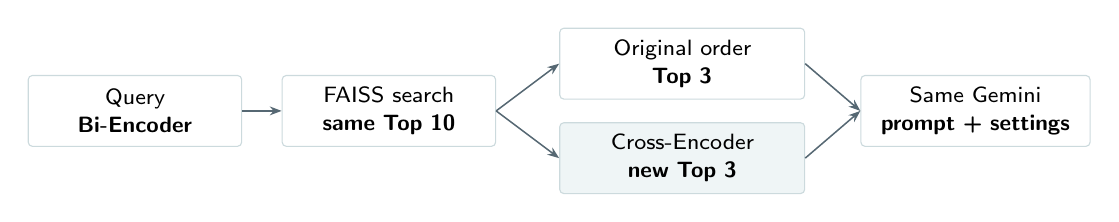
\begin{tikzpicture}[font=\sffamily\fontsize{8.3}{10}\selectfont,
 stage/.style={draw=line,fill=white,rounded corners=1.5pt,align=center,minimum height=9mm,text width=25mm,inner sep=3pt},
 route/.style={-{Stealth[length=1.5mm]},draw=muted,line width=0.55pt}]
\node[stage] (query) {Query\\\textbf{Bi-Encoder}};
\node[stage,right=5mm of query] (ten) {FAISS search\\\textbf{same Top 10}};
\node[stage,right=8mm of ten,yshift=6mm,text width=29mm] (base) {Original order\\\textbf{Top 3}};
\node[stage,right=8mm of ten,yshift=-6mm,text width=29mm,fill=pale] (cross) {Cross-Encoder\\\textbf{new Top 3}};
\node[stage,right=7mm of base,yshift=-6mm,text width=27mm] (llm) {Same Gemini\\\textbf{prompt + settings}};
\draw[route] (query)--(ten);
\draw[route] (ten.east)--(base.west);
\draw[route] (ten.east)--(cross.west);
\draw[route] (base.east)--(llm.west);
\draw[route] (cross.east)--(llm.west);
\end{tikzpicture}
\end{center}
\vspace{-5pt}
Baseline supplies the original first three candidates to Gemini. The Cross-Encoder, \texttt{ms-marco-MiniLM-L6-v2}, jointly processes all ten query--chunk pairs, allowing self-attention across their tokens [3, 4]. It sorts by descending relevance score and selects a new Top~3. Its scores are neither probabilities nor cosine similarities.

Both answers use \texttt{gemini-3.8-flash}, temperature~0, seed~42, and the same evidence-and-citation prompt template [5]. Only the selected excerpts change. These settings do not guarantee deterministic generation.
\section{Qualitative and rank shift analysis}
Five cases were selected from 44 exploratory queries. The three recoveries were checked for equivalent evidence across the full baseline context. They are selected stress tests, not an estimate of average accuracy. The six paired answers below are reproduced in full.
\casetitle{D10}{Resetting failed attempts}{Rank 4 $\rightarrow$ 1}
\question{When a user requests a fresh out-of-band verification code, can the failed-attempt counter start over?}
\location{PDF 33 / printed 22; section 3.1.3.2. Tracked chunk: \chunk{p033\_c03}.}
\begin{response}{line}
\answerlabel{ANSWER 1 / BASELINE}
The provided excerpts do not establish whether a failed-attempt counter can start over when a user requests a fresh out-of-band verification code. The excerpts discuss out-of-band authenticators and recovery code requirements, including validity periods, format, and throttling under Sec. 3.2.2 [p059\_c03, p031\_c04, p059\_c02], but they completely lack any mention of a failed-attempt counter or the conditions under which it may be reset.
\end{response}
\begin{response}{teal}
\answerlabel{ANSWER 2 / RERANKED}
No. Generating a new authentication secret SHALL NOT reset the failed authentication count [p033\_c02, p033\_c03].
\end{response}
\note{Baseline returned recovery-code material rather than the counter restriction. Reranking changes an explicit abstention into a supported answer; it does not correct a fabricated reset rule.}
\newpage
\vspace*{1pt}
{\sffamily\fontsize{9}{11}\selectfont\bfseries\color{teal}QUALITATIVE ANALYSIS / CONTINUED}\par\vspace{3pt}
\casetitle{D28}{Reusing biometric samples}{Rank 5 $\rightarrow$ 2}
\question{Can face images collected during sign-in be reused to improve the matching template or for research, and what permission is needed?}
\location{PDF 45 / printed 34; section 3.2.3.4. Tracked chunk: \chunk{p045\_c01}.}
\begin{response}{line}
\answerlabel{ANSWER 1 / BASELINE}
The provided excerpts do not establish whether face images collected during sign-in can be reused to improve the matching template or for research, nor do they establish what permission is needed.

The excerpts only state that facial images do not constitute secrets and can often be obtained without consent [p043\_c01], detail usability considerations that affect facial recognition accuracy (e.g., artifacts, lighting, expressions, poses) [p089\_c01], and define central comparison requirements\textemdash{}including that sensors/endpoints SHALL be authenticated, appropriate controls SHALL be implemented for sensitive personal information, and verifiers MAY limit centrally stored templates to particular sensors [p044\_c04]. Any provisions regarding the reuse of sign-in biometric samples or required permissions are missing.
\end{response}
\begin{response}{teal}
\answerlabel{ANSWER 2 / RERANKED}
Biometric samples collected during the authentication process MAY be used locally within the authenticator or verifier performing the biometric comparison to update templates (to compensate for changes in subscriber characteristics) or for other research purposes [p045\_c01].

Regarding permission:
\begin{itemize}[leftmargin=1.3em,itemsep=1pt,topsep=2pt]
\item For research purposes, "explicit subscriber consent" is required [p045\_c01].
\item For updating templates to compensate for changes in subscriber characteristics, the text does not state that permission is needed [p045\_c01].
\end{itemize}

Additionally, the samples and any derived biometric data SHALL be erased immediately after adaptation or research data has been derived, and an allowable time limit for adaptation SHALL be established and enforced by the authenticator or CSP [p045\_c01].
\end{response}
\note{Baseline lacked the reuse and consent clause. Reranking restores local use and explicit subscriber consent for other research. The provision does not state that template adaptation needs consent; this does not establish an exemption from all other applicable consent requirements.}
\vspace{7pt}
{\color{line}\hrule height 0.35pt}\vspace{4pt}
\casetitle{D34}{Sending a postal recovery notice}{Rank 6 $\rightarrow$ 1}
\question{If the only electronic notification address was also used to receive a recovery code, can the provider skip sending a postal recovery notice?}
\location{PDF 63 / printed 52; section 4.6. Tracked chunk: \chunk{p063\_c02}.}
\begin{response}{line}
\answerlabel{ANSWER 1 / BASELINE}
The provided excerpts do not establish the answer. They do not contain any information or requirements regarding postal recovery notices, nor do they state whether a provider can skip sending a postal recovery notice if the only electronic notification address was used to receive a recovery code [p059\_c02, p059\_c03, p060\_c01].
\end{response}
\begin{response}{teal}
\answerlabel{ANSWER 2 / RERANKED}
No, the provider cannot skip sending a postal recovery notice [p063\_c02].

According to the excerpt, account recovery notifications SHALL also be sent to a postal address if the only other notification address in the subscriber account is the address to which an issued recovery code was sent [p063\_c02].
\end{response}
\note{Baseline covers recovery-code delivery, omitting the notification exception. Reranking restores the separate postal-notice obligation when the only other notification address received the issued recovery code.}
\newpage
\smallhead{Controls and retrieval limits}
\textbf{D03 / equivalent evidence.} The AAL3 prohibition for cloud-synced passkeys, \chunk{p020\_c01} (PDF~20, printed~9, section~2.3.2), moves from rank~4 to~2. But baseline rank~2 already contains equivalent evidence in \chunk{p103\_c02} (PDF~103, printed~92). Both answers correctly reject synced passkeys at AAL3. This is not a failure recovery.

\textbf{D05 / candidate recall.} The voice-biometric prohibition in \chunk{p043\_c04} (PDF~43, printed~32, section~3.2.3.2) is absent from the initial Top~10. Baseline incorrectly permits voice biometrics under general biometric conditions; the reranked answer abstains. This avoids unsupported permission without recovering the missing rule. Full control answers and candidate lists remain in the notebook and results.
\section{Latency profiling}
Each query has one warm-up and seven measured repetitions: \textbf{35 samples}. The run uses Python~3.12.3 on an ARM64 Mac with macOS~26.6.2, CPU inference, and one thread each for Torch and FAISS. Table~1 reports medians from \texttt{results/latency\_summary.csv}.
\begin{center}
\small
\setlength{\tabcolsep}{9pt}
\begin{tabularx}{\linewidth}{>{\bfseries}l *{3}{>{\raggedleft\arraybackslash}X} >{\raggedleft\arraybackslash}p{23mm}}
\toprule
\rowcolor{pale}
\normalfont\sffamily\bfseries Case & \sffamily\bfseries Baseline & \sffamily\bfseries Reranking & \sffamily\bfseries Advanced & \sffamily\bfseries Total /\\[-1pt]
\rowcolor{pale}
& \sffamily\bfseries (ms) & \sffamily\bfseries increment (ms) & \sffamily\bfseries total (ms) & \sffamily\bfseries baseline\\
\midrule
D10 & 4.70 & 127.72 & 132.14 & 28.11$\times$\\
D28 & 4.76 & 125.96 & 130.72 & 27.46$\times$\\
D34 & 4.64 & 125.72 & 130.52 & 28.16$\times$\\
D03 & 4.68 & 124.72 & 129.50 & 27.69$\times$\\
D05 & 4.85 & 133.90 & 138.65 & 28.60$\times$\\
\bottomrule
\end{tabularx}\par\vspace{4pt}
{\fontsize{8.5}{10.5}\selectfont\color{muted}\textbf{Table 1.} Retrieval latency; model loading, PDF processing, indexing, and Gemini generation are excluded.}
\end{center}
\vspace{-4pt}
Baseline includes query embedding, vector search, and candidate construction. The reranking increment includes pair validation, tokenization, inference, sorting, and result construction. Advanced total adds both stages \emph{within each repetition}; separate medians need not sum exactly.

Advanced retrieval takes about \textbf{27.5--28.6 times as long} here. Seven samples offer limited precision. The latest run recomputed retrieval and timings but reused all ten earlier Gemini responses from an exact prompt/model/configuration cache, with \textbf{zero fresh API answers}. Original response timestamps are retained in \texttt{results/answers.json}.
\section{Why reranking follows retrieval}
A Cross-Encoder must jointly process every query--chunk pair. Scoring the whole corpus would require \textbf{409 pairs rather than ten}: 40.9 times as many pairs, \emph{not} a measured 40.9-fold latency increase. Bi-Encoder document vectors are reused across queries; the vector store restricts expensive joint scoring to ten candidates. This implementation uses exact FAISS search, rather than approximate search.

Pair counts grow with the collection. D05 exposes the trade-off: an initial retrieval miss prevents reranking from restoring the absent rule. Reranking improves selection only within the candidates it receives.
\vspace{4pt}
{\color{line}\hrule height 0.35pt}\vspace{3pt}
\smallhead{References}
{\fontsize{8.7}{11.2}\selectfont
\setlength{\parskip}{2pt}
[1] NIST. \href{https://csrc.nist.gov/pubs/sp/800/63/b/4/final}{SP 800-63B-4: Authentication and Authenticator Management}. Final, July 2025.\par
[2] Sentence Transformers. \href{https://huggingface.co/sentence-transformers/all-MiniLM-L6-v2}{\texttt{sentence-transformers/all-MiniLM-L6-v2} model card}.\par
[3] Cross-Encoder. \href{https://huggingface.co/cross-encoder/ms-marco-MiniLM-L6-v2}{\texttt{cross-encoder/ms-marco-MiniLM-L6-v2} model card}.\par
[4] Sentence Transformers. \href{https://www.sbert.net/docs/cross_encoder/usage/usage.html}{Cross-Encoder usage documentation}.\par
[5] Google AI for Developers. \href{https://ai.google.dev/gemini-api/docs/generate-content}{Gemini content generation documentation}.\par
}
\end{document}
